\documentclass{../Skript}

\begin{document}
\section{Numerische Integration}
Berechnung von Integralen, z.B. zur Flächen- oder Volumenberechnung, 
aber auch 
notwendig in komplexeren Formeln/Algorithmen, z.B. Fourier-Integrale, 
Numerik 
partieller-Differentialgleichungen. Oft nicht (leicht) von Hand zu 
berechnen, 
\(\Rightarrow\) Algorithmen zur näherungsweisen Berechnung von 
Integralen.\\
Viele typiche ''\underline{Quadraturformeln}'' haben für \(f\in C[a,b]\)
die Form 
\[
\int^b_a f(x)\, dx \approx \sum_{i=0}^n x_i f(x_i),
\]
 d.h. Kombination von Punktauswertungen mit Stützstellen \( a\leq x_0 < 
 x_1\dots 
 x_n\leq b\)
\begin{remindexample}[Rieman-Integral]\hfill\\
z.B. Rieman-Summe \[
I_h(f)\coloneqq \sum_{i=1}^n f(x_{i-1})\cdot(x_i-x_{i-1})
\]
\(f\) Rieman-Integrierbar \(\leadsto I_h(f)\to I(f) \text{ für } h\to 
0, \ 
h\coloneqq \max(x_i-x_{i-1})\)\\
\end{remindexample}
\subsection{Interpolatorische Quadraturformel}
Kennt man eine Polynom-Interpolation von $f$, (oder Hermite-), kann man 
statt $f$ 
einfach die Interpolierende integrieren. Integration über Polynome ist 
einfach.
Zu \(a\leq x_0 <x_1\dots < x_n\leq b\) sei \(P_n\in\bbP_n\) das 
interpolierende 
Polynom zu \(f\) mit \(P_n(x_i)=f(x_i), i=0,\dots, n\)\\
setze dann \[
I^{(n)}(f)\coloneqq \int^b_aP_n(x)\, dx =\int^b_a \sum_{i=0}^n 
f(x_i)L^{(n)}_i(x)\, dx = \sum_{i=0}^n f(x_i)\int^b_a L^{(n)}_i(x)\, dx
\]
\[
P_n(x)=\sum_{i=0}^n f(x_i)L^{(n)}_i(x)
\]
Wie groß ist der Fehler \(I(f)-I^{(n)}\)?\\
Mit der Formel fürden Interpolationen Fehler folgt:

\begin{theorem}
    Für die Lagrange-Quadraturformel $I^{(n)}$ gilt, falls $f \in
    C^{n+1}[a,b]$:\[
        I(f) - I^{(n)}(f) = \int_a^b f(x) - p_n(x) dx = \int_a^b\frac{1}
        {(n+1)!}
        f^{(n+1}(\xi_x)\prod_{j=0}^n(x-x_j)dx
    \]
    also \[   
        \abs{I(f) - I^{(n)}(f)} \leq \frac{1}{(n+1)!}\cdot 
        \max\limits_{[a,b]}
        \abs{f^{(n+1)}}\cdot \abs{\int_a^b\prod_{j=0}^n(x-x_j) dx}
    \]
\end{theorem}
\begin{remark}
    man kann auch zeigen:\[
    I(f) - I^{(n)}(f) = \int_a^b f[x_0, \dots, x_n, x] \prod_{j=0}^n(x-
    x-j)dx
    \] 
\end{remark}

Interpolatorische Integrationsformeln, \(I^{(n)}
(f)\coloneqq\int^b_ap_n(x)\diff 
x\), \( p_n\in\bbP\) des Interpolationspolynoms zu \(f\) in  
\(x_0,\dots,x_n
\in[a,b]\) Nach Konstruktion: die interpolierende Quadraturformel ist 
''exakt'' 
für beliebige Polynome \(p\in\bbP_n\), wegen des Eindeutigkeit der 
Interpolationspolynoms.
\begin{definition}
    Eine Quadraturformel \(I^{(n)}\) wird (mindestens) ''\underline{von 
    der 
    Ordnung m}'' genannt, falls durch sie alle Polynomevom Grad \(\leq 
    m-n\) 
    exakt integriert werden.
\end{definition}
Damit sind die interpolatorischen Quadraturformeln \(I^{(n)}\) 
mindestens von der 
Ordnung \(n+1\).

\begin{example}[Lagrange-Quadraturen mit n+1 Stützstellen mit gleichen 
Abständen]\hfill
\begin{enumerate}[(a)]
    \item ''(abgeschlossene) \underline{Newton-Cotes-Formeln}'':\\
    $a,b$ sind Stützstellen, $x_i=a+ih,\midspace \igb i 0 n$ mit 
    $h=\frac{b-a}{n}$
    \item ''\underline{offene Newton-Cotes-Formeln}:\\
    $a,b$ sind \underline{keine} Stützstellen, $x_i = a+(i+1)h,\midspace
    \igb i 0 
    n, \midspace h=\frac{b-a}{n+2}$
\end{enumerate}
Die ersten Newton-Cotes-Formeln sind:
\begin{description}
\item[abgeschlossen:]\begin{align*}
    I^{(1)} &= \frac{b-a}{2}(f(a) + f(b)) && 
    \text{''\underline{Trapezregel}''}\\
    I^{(2)} &= \frac{b-a}{6}\left(f(a) + 4f\left(\frac{ab}{2}\right) + 
    f(b)\right) && \text{''\underline{Keplersche Fassregel}''}\\
    I^{(3)} &= \frac{b-a}{8}\left(f(a) + 3f(a+h) + 3f(b-h) + f(b)\right)
    && 
    \text{''\underline{$\frac{3}{8}$-Regel}''}
\end{align*}    
\item[offen:]\begin{align*}
    I^{(0)}(f) &\coloneqq (b-a) \cdot f\left(\frac{a+b}{2}\right) && 
    \text{''\underline{Mittelpunktsregel}''}\\
    I^{(1)}(f) &\coloneqq \frac{b-a}{2}(f(a+h) + f(b-h))\\
    I^{(2)}(f) &\coloneqq \frac{b-a}{3}\left(2f(a+h) - f\left(\frac{a+b}
    {2}\right) + 2f(b-h)\right)  
\end{align*}

\end{description}
\end{example}
Mit den Interpolationsabschätzungen und Integral-Mittelwertsätzen zeigt 
man:

\begin{theorem}[Quadraturfehler Newton-Cotes-Formeln]\hfill
    \begin{enumerate}[i)]
        \item Für die Trapezregel \(I^{(1)}\) mit \(f\in C^2[a,b]\) 
        gilt: \[
        \int^b_af(x)\diff x-\frac{b-a}{2}(f(a)+f(b)) = -\frac{(b-
        a)^3}{12}f''(\xi) \text{ mit } \xi\in[a,b]
        \]
        \item Für die Simpson-Regel \(I^{(2)}\) mit \(f\in C^4[a,b]\) 
        gilt: \[
        \int^b_af(x)\diff x-\frac{b-a}{2}(f(a)+4f(\frac{a+b}{2})+f(b)) 
        = 
        -\frac{(b-a)^5}{2880}f^{(4)}(\xi) \text{ mit } \xi\in[a,b]
        \]
        \item Für die Mittelpunktformel \(I^{(0)}\) mit \(f\in 
        C^2[a,b]\) gilt: \[
        \int^b_af(x)\diff x-(b-a)f(\frac{a+b}{2} = -\frac{(b-
        a)^3}{24}f^{(2)}(\xi) \text{ mit } \xi\in[a,b]
        \]
    \end{enumerate}
\end{theorem}
\begin{proof}
    zu i) \begin{align*}
    \int^b_af(x) \diff x - \int^b_a p_n(x) \diff x &= \int^b_a f(x)-
    p_n(x) \diff 
    x\\
    &=\int^b_a f''(\xi(x))\cdot \frac{1}{2}\cdot(x-a)(x-b)\diff x\\
    &= f''(\xi)\frac{1}{2}\int^b_a(x-a)(x-b)\diff x\\
    &= \frac{1}{12}f''(\xi)(b-a)^3
   \end{align*}
\end{proof}
\begin{remark}
    zu iii) Mittelpunktformel ist exakt nicht nur für \(p\in\bbP_0\) 
    sondern 
    sogar für alle \(p\in\bbP_n\)
\end{remark}

\begin{remark}
    Sind neben $f$ auch die Ableitungen $f'(x)$ bekannt, dann kann man 
    auch eine 
    Hermite-Interpolation zur Herleitung von Quadraturformeln nehmen, 
    die Hermite-
    Interpolationsfehlerabschätzung überträgt sich dann auf die 
    Quadraturfehlerabschätzung.
\end{remark}
Um ein Integral besser zu approximieren, wird typicherweise nicht der 
Polynomgrad 
weiter erhöht, sondern eine Quadraturformel mit relativ geringen Grad 
auf 
Teilintervallen immer kleinerer Größe genutzt:\\
z.B.    $a = y_0 < y_1 < \dots < y_N = b$ mit Teilintervallen $I_i = 
[y_{i-1}, 
    y_i]$:\[
        \int_a^b f(x)\diff x = \sum_{i=1}^N \int_{I_i}f(x)\diff x\approx
        \underset{I_h^{(n)}(f)}{\underbrace{\dsum_{i=1}^N \int_{I_i} 
        \underset{\text{Interpolierende}}
        {\underbrace{I^{(n)}_{[y_{i-1}, y_i]}f}}\diff x}}
    \] 
    und \begin{align*}
                \int_a^b f(x)\diff x - I_h^{(n)}(f) &= \dsum_{i=1}^N 
                \int_{I_i}f(x)\diff x - \int_a^b\left(I_{[y_{i-1}, 
                y_i]}^{(n)}f\right)(x)\diff x\\
                &\leq \dsum_{i=1}^N c_m\cdot(y_{i-1}-
                y_i)^{m+1}\abs{f^{(m)}
                (\xi_i)}\\
                &\leq \dsum_{i=1}^N c_mh^{m+1}\cdot 
                \dabs{f^{(m)}}_{\max[a,b]}\\
                &\leq c_m(b-a)\frac{h}
                {h_{\min}}h^{m}\cdot\dabs{f^{(m)}}_{\max}
    \end{align*}
    mit \[
        N\leq \frac{b-a}{h_{\min}} , \largespace \frac{h}{h_{\min}}= 1, 
        \text{ 
        falls 
        alle Teilintervalle gleich lang sind}
    \]
\begin{example}
    $y_i = a+ih, \largespace h=\frac{b-a}{N}, \largespace \igb i 0 N$ 
    gleichgroße 
    Teilintervalle. 
    Summierte Trapezregel \begin{align*}
        I^{(1)}_h(f)\coloneqq \frac{h}{2}\left(f(a)+ \dsum_{i=1}^{N-
        1}2f(y_i)+f(b)\right), \\
        \abs{I(f)-I^{(1)}_h(f)}\leq \frac{b-a}{12}h^2
        \abs{\abs{f^{(2)}}}_{\max[a,b]}
    \end{align*}
    Summierte Simpsonregel: \begin{align*}
        I^{(2)}_h(f)\coloneqq \frac{h}{6}\left(f(a)+ \dsum_{i=1}^{N-
        1}2f(y_i)+\dsum_{i=1}^{N}4f\middle(\frac{y_{i-1}+y_i}
        {2}+f(b)\middle)
        \right), \\
        \abs{I(f)-I^{(2)}_h(f)}\leq \frac{b-a}{2880}h^4
        \abs{\abs{f^{(4)}}}_{\max}
    \end{align*}
    Summierte Mittelpunktregel: \begin{align*}
        I^{(0)}_h(f)\coloneqq h\dsum_{i=1}^{N}f\left(\frac{y_{i-1}+y_i}
        {2}\right), \\
        \abs{I(f)-I^{(0)}_h(f)}\leq \frac{b-a}{24}h^2
        \abs{\abs{f^{(2)}}}_{\max}
    \end{align*}
\end{example}
\begin{remark}
    Ähnlich geht es für Hermite-Splines, d.h. lokale Hermite-
    Interpolierende
\end{remark}
\begin{motivation}
    Mittelpunktsregel und Simpson-Regel sind von höherer Ordnung als 
    man es durch 
    den Polynomgrad alleine erwarten würde, anscheinend allein durch 
    die 
    geschickte Wahl der Stützstellen. 
\end{motivation}
\begin{question}
    Wie gut kann man werden bei optimaler Wahl der Stützstellen?
\end{question}
\subsection{Gauß-Quadraturformeln}
Man sieht leicht, dass die Maximale Ordnung einer interpolierenden 
Quadraturformel nach oben begrenzt ist
\begin{lemma}
    Eine obere Grenzen für die Ordnung einer interpol. Quadraturformel 
    $I^{(n)}$ 
    mit $n+1$ Sützstellen ist $2n+2$
\end{lemma}
\begin{proof}
    Wäre Ordnung höher, könnte man alle Polynome vom Grad $2n+2$ exakt 
    integrieren. Für das Polynom \[
        p(x) \coloneqq \prod_{i=0}^n(x-x_i)^2 \in \bbP_{2n+2}
    \]
    gilt \[
    \forall \igb i 0 n: p(x_i) = 0
    \]
    also \[
        I^{(n)}(p) = 0
    \]
    da \[
        I^{(n)}(p) = \dsum_{j=0}^n w_ip(x_i)
    \]
    aber \[
    \forall x: p(x) \geq 0, \text{ also }p\not\equiv 0
    \]  
    demnach \[
        \int_a^b p(x)\diff x > 0 \lightning
    \]    
\end{proof}
Man kann bei geschickter Wahl der Stützstellen also alle Polynome $p\in\bbP_{2n+1}$ exakt integrieren.
%%%%%%%%%%%%%%%%%%%%%%%%%%%%%%%%%%%%%%%%%%%%%%%%%%%%%%%%%%%%%%%%%%%%%%%%%%%%%
Ein Polynom $p\in\bbP_{2n+1}$ kann man immer zerlegen in \[
    p(x) = r(x) \cdot q(x) + s(x)\]
mit $q\in \bbP_{n+1}$ fest vorgegeben, $\deg{q} = n+1$, $r,s\in \bbP_n$.
Z.B. für $q(x) =x^{n+1}$: \[
    p(x) = \dsum_{i=0}^{2n+1}a_ix^i \implies r(x) = \sum_{i=0}^n a_{i+n+1}x^i, \largespace s(x) = \sum_{i=0}^na_i^i\]
für eine Wahl $a \leq x_0 < x_1 < \dots < x_n \leq b$ wählen wir \[
    q(x) \coloneqq \prod_{i=0}^n(x-x_i) \in \bbP_{n+1}\]
\begin{question}Quadraturformel für $p$?
\end{question}
Es ist \begin{align*}
    \int_a^b p(x) \diff x &= \underset{I^{(n)}(r\cdot q) + \text{ Rest}}{\underbrace{\int_a^b r(x) q(x) \diff x}} + \underset{I^{(n)(s)}}{\underbrace{\int_a^b s(x)\diff x}}
\end{align*}
Falls also \[
    \int_a^b p(x) \diff x \overset{!}{=}I^{(n)}(p)\]
sein soll für alle $p\in\bbP_{2n+1}$, dann muss \[
    \int_a^b r(x) q(x) \diff x = 0 \text{ für alle $r\in \bbP_n$}\]
\begin{question}
    gibt es ein $q\in \bbP_{n+1}$, bzw \[x_0 < \dots < x_n \in [a,b], \midspace q(x) = \prod_{i=0}^n(x-x_i)\]
    so, dass \[
        \int_a^b r(x)q(x)\diff x = 0\]
    für alle $r\in \bbP_n$?
\end{question}
Wir betrachten den Raum $\bbP_{n+1}$ mit Basis $\set{1,x,x^2,\dots,x^{n+1}}$ mit
\underline{Skalarprodukt} \[
    (r,q)\coloneqq \int_a^b r(x)q(x)\diff x\midspace \text{für alle }r,q\in\bbP_{n+1}\]
\underline{Gram-Schmidt-Orthogonalisierungsverfahren}:\[p_0(x) \coloneqq 1, \largespace
p_n(x) \coloneqq x^k - \dsum_{j=0}^{k-1}\frac{\left(x^k, p_j\right)}{\left(p_j,p_j\right)}p_j, \largespace \igb k 1 {n+1}\]
%Die Klammern, damit außerhalb von diesem Block der alte Skalarprodukt Makro bleibt
{
\def\scp#1#2{\ensuremath{\left(#1,\ #2\right)}}
Also steht $p_{n+1}$ senkrecht auf $\lin{p_0, \dots, p_n} = \bbP_n$, d.h. \[
    \scp r {p_{n+1}} = 0 \largespace\forall r \in \bbP_n
    \]
    dementsprechend ist $p_{n+1}$ Kandidat für unser Polynom $q$, $q = p_{n+1}$, da
    die führende Potenz $1\cdot x^{n+1}$ die gleiche ist. Mann kann zeigen, dass alle
    $p_k$ jeweils $k$ verschiedene, einzelne Nullstellen hat, damit $q=\bbP_{n+1}$ gerade
    Nullstellen $x_i$, $a\leq x_0 < \dots < x_n \leq b$ hat, und damit \[
        q(x) = \prod_{i=0}^n(x-x_i)\]
\begin{theorem}[''Gauß-Quadratur'']\hfill\\
    Es gibt genau eine interpolatorische Quadraturformel zu $n+1$ paarweise verschiedene Stützstellen
    über dem Intervall $[-1, 1]$ mit der optimalen Ordnung $2n+1$. Die zugehörigen Sützstellen
    sind die Nullstellen des $(n+1)$-ten Legendrepolynoms $L_{n+1}\in \bbP_{n+1}$, und die Gewichte sind\[
        w_i = \int_{-1}^1 \prod_{j\neq i}(x-x_j)^2 \diff x > 0\]
    Für $f\in C^{2n+1}[-1,1]$ ist der Quadraturfehler \[
        \int_a^b f(x)\diff x - \sum_{i=0}^n w_if(x_i) = \frac{1}{(2n+2)!}f^{(2n+2)}(\xi)\int_{-1}^1\prod_{i=0}^n(x-x_i)^2\diff x\]
\end{theorem}
\def\LgBp#1#2{\ensuremath{L_{#1}^{(#2)}}}
\begin{proof}
    \begin{description}
        \item[gewichte $\mathbf{w_i}$:]
         Sei $L_i^{(n)}$ das $i$-te Lagrange-Basispolynom \[
        \frac{\dprod_{j\neq i}(x-x_j)}{\dprod_{j\neq i}(x_i-x_j)}\in\Pol{n}\]
    \[L^{(n)}_i(x_j) = \delta_{ij} = \begin{cases}
        1 & i=j\\0&\text{sonst}
    \end{cases}\] Damit ist $\left(L_i^{(n)}\right)^2 \in \Pol{2n}$, und Gauß-Quadraturformel exakt\begin{align*}
        \int_{-1}^1 \left(L_i^{(n)}\right)^2 \diff x &= \sum_{j=0}^n w_j\cdot  {\LgBp{i}{n}}^2(x_j) \\
        &= \sum_{j=0}^n w_j \cdot \delta_{ij} = w_i
    \end{align*}
    Also ist $w_i > 0$
    \item[Eindeutigkeit:]
    ergibt sich aus Orthogonalität von $q$ zu $\Pol{n}$, orthogonaler Unterraum ist $1-$dimensional,
    alle Vielfachen eines Polynoms $\neq 0$, damit haben alle Polynome des orthog. Unterraums
    die gleichen Nullstellen
    \item[Fehlerabschätzung:]
    Wir nutzen eine Hermite-Interpolation als Hilfsmittel. Zu $f\in C^{2n+2}[-1,1]$ sei
    $h \in \Pol{2n+1}$ die Hermite-Interpolierende zu $f(x_i), \ f'(x_i), \ \igb i 0 n$. Dafür hatten
    wir die Abschätzung\[
        f(x) - h(x) = \frac{1}{(2n+2)!} f^{(2n+2)}(\xi_x)\cdot\prod_{i=0}^n (x-x_i)^2\]
    Damit ist 
    \begin{align*}
        I(f) - I^{(n)}(f) &= \left(I(f) - I(h)\right) - \left(I^{n}(f) - \underset{I^{(n)}(h)}{\underbrace{I(h)}}\right)\\
        &= \int_{-1}^1 f(x)-h(x)\diff x - \sum_{i=0}^n w_i\underset{=0}{\underbrace{(f(x_i) - h(x_i))}}\\
        &= \int_{-1}^1 \frac{1}{(2n+2)!}f^{(2n+2)}(\xi_x)\cdot\prod(x-x_i)^2\diff x\\
        &\overset{\text{MWS}}{=} \frac{1}{(2n+2)!}f^{(2n+2)}(\xi)\cdot\prod_{j=0}^n(x-x_i)^2
    \end{align*}
    \end{description}
\end{proof}
\underline{''Legendre-Polynome''}:\\
    $L_k(x)$, Orthogonalpolynome bzgl. \[\scp{r}{s} = \int_{-1}^1 r(x)s(x)\diff x\]
    Es ist \[
        L_0(x) \equiv 1, \midspace L_1(x) = x, \midspace (k+1)L_{k+1}(x) = (2k+1)x\cdot L_k(x) - kL_{k-1}(x)\]
    also \[
        L_2(x) = \frac{1}{2}(3x^2 - 1) = \frac{3}{2}x^2 - \frac{1}{2}\]
    Eine andere Formel ist \[
        L_k(x) = \frac{1}{2^k\cdot k!}\frac{d^k}{dx^k}\left((x^2-1)^k\right)\]
\begin{remark}
    Analoges Vorgehen bei Integration mit einer Gewichtsfunktion \[
        w(x): \ I_w(f) \coloneqq \int_a^b f(x)\cdot w(x)\diff x\]
    Orthogonalisierung bzgl des gewichteten Skalarprodukts \[
        \scp{r}{s}_w \coloneqq \int_a^b r(x)\cdot s(x)\cdot w(x)\diff x, \largespace w>0\text{ fast überall, z.B. stetig}\]
\end{remark}
\begin{example}
    Für $w(x) \coloneqq \frac{1}{\sqrt{1-x^2}}$ auf $[-1,1]$ ergeben sich als Orthogonalpolynome 
    gerade die Tschebyscheff Polynome $T_k(x)$.\\
    Für $w(x)\equiv 1$: Legendre-Polynome, s.o.
\end{example}
\underline{Für Integration auf dem Intervall $[a,b]$}: Transformation \[[-1,1]\to [a,b],\largespace \int_a^b f(x)\diff x = 
\frac{b-a}{2}\int_{-1}^1 f\left(\frac{a+b}{2}+ t\frac{b-a}{2}\right)\diff t\] 
Um Integrale genauer zu berechnen, wird auch bei den Gauß-Formeln nicht unbedingt der
Polynomgrad weiter erhöht so, dass wieder eine Summe über kleinere Teilintervalle $I_j, \igb j 1 N$ genutzt,
$I_j = [y_{j-1}, y_j], \midspace a=y_0< y_n \dots < y_N = b$
Und für jedes Teilintervall die entsprechend transformierte Quadraturformel. Dafür bekommt man
dann eine Fehlerabschätzung \begin{align*}
        \abs{I(f) - I_h^{n}(f)} &= \abs{\int_a^b f(x)dx - \sum_{j=1}^N \frac{y_j-y_{j-1}}{2}\cdot \left(\sum_{i=0}^n w_i \cdot \Tilde{f_j}(x_i)\right)}\\
        &\leq (b-a)\cdot c \cdot h^{2n+2}\cdot \dabs{f^{(2n+2)}}_{\max[a,b]}
    \end{align*}
    mit $h\coloneqq \max_{\igb j 1 N}(y_j-y_{j-1})$. Dabei ist $c$ unabhängig von $a,b,h,f$.
    Bei Halbierung der Teilintervalllängen reduziert sich der Quadraturfehler also um 
    Faktor $\left(\frac{1}{2}\right)^{2n+2}$.
% WIR MÜSSEN IN DIE KLAMMER SCHREIBEN
\subsection{Richardson-Extrapolation}
Eine Idee/Methode, die man auch in anderen Situationen gut und gerne anwenden 
kann:\\
Angenommen Berechnungsvorschrift mit Diskretisierungsgröße $h > 0$, $h\searrow 0$
so, dass wir für die Approximation einer Größe $E_0$ eine \underline{Entwicklung}
der berechneten Größe $E(h)$ haben der Form \[
    E(h)  = E_0 + c_1h^{K_1}+c_2h^{K_2} \in \calO{h^{K_2}}\text{ mit }0<k_1<k_2
\] 
Dann können wir Berechnungen mit zwei verschiedenen qDiskretisierungen $h_1 > h_2 
> 0$ durchführen, und mit diesen Ergebnissen die Ordnung $h^{K_1}$ eliminieren
\begin{align*}
    E(h_1)&=E_0+c_1h_1^{K_1}+c_2h_1^{K_2}\qquad \vert\cdot h_2^{K_1}\\
    E(h_2)&=E_0+c_1h_2^{K_1}+c_2h_2^{K_2}\qquad \vert\cdot h_1^{K_1}\\
    h_1^{K_1}E(h_2)-h_2^{K_1}E(h_1)&=(h_1^{K_1}-h_2^{K_1})E_0+c_1\cdot0+c_2(h_1^{K_1}h_2^{K_2}-h_2^{K_1}h_1^{K_2})\\
    \frac{ h_1^{K_1}E(h_2)-h_2^{K_1}E(h_1)}{h_1^{K_1}-h_2^{K_1}}&= E_0+c_2\frac{h_1^{K_1}h_2^{K_2}-h_2^{K_1}h_1^{K_2}}{h_1^{K_1}-h_2^{K_1}}\\
    \intertext{\(h_2=dh_1\)}
    \frac{h_1^{K_1}(E(h_2)-d^{K_1}E(h_1))}{h_1^{K_1}(1-d^{K_1})}&= E_0+c_2\frac{(d^{K_2}-d^{K_1})h_1^{K_1+K_2}}{h_1^{K_1}(1-d^{K_1})}\\
    \Rightarrow \frac{E(h_2)-d^{K_1}E(h_1)}{1-d^{K_1}}&= E_0+c_2\frac{d^{K_2}-d^{K_1}}{1-d^{K_1}}h_1^{K_2}
\end{align*}
Durch geschickte Kombination erhalten wir eine Approximation der Ordnung \(\calO{h^{K_2}}\) auch ohne \(K_2\) explizit zu kennen.

%%%%%%%%%%%%%%%%%%%%%%%%%%%%%%%%%%%%%%%%%%%%%%%%%%%%%%%%%%%%%%%%%%

\subsubsection*{Anwendung auf numerische Integration}
Wir kennen (falls die uzu integrierende Funktion glatt genug ist) die führenden
Ordnungen des Quadraturfehlers vieler interpolierender Quadraturformeln. Durch 
geeignete Kombination von Integrationen mit gleichlangen Teilintervallen mit 
Längen $h_1, h_2$ erreicht man dann eine Approximation des Integrals $I(f)$ von 
besserer Ordnung. Hat man eine weitergehende Entwicklung wie \[
    E(h) = E_0 + c_1h^{K_1} + c_2 h^{K_2} + c_3h^{K_3}\dots\]
können entsprechend auch weiter höhere Ordnungen eliminiert werden, indem 
genügend verschiedene Berechnungen mit verschiedenen $h$'s durchgeführt werden. 
\begin{example}
    \hfill
    \begin{center}
        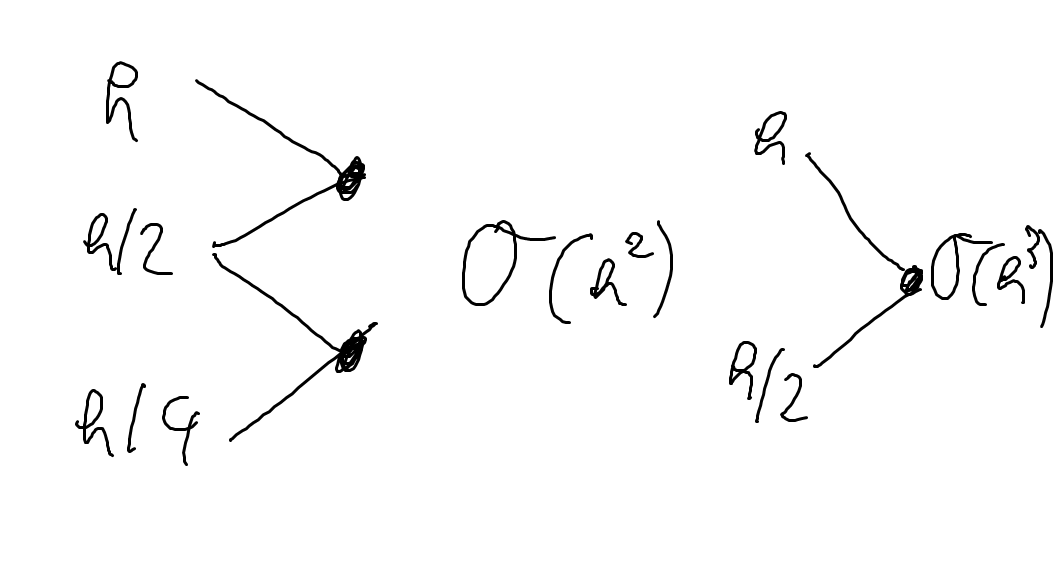
\includegraphics[width=\linewidth]{../Bilder/051222_1.png}
    \end{center}
\end{example}
%%%%
Für die summierte Trapezregel auf einer gleichmäßigen Zerlegung mit Teilintervallen der Länge \(h=\frac{b-a}{N},\ x_i=a+ih,\ i=1,\dots,N\)
kann man zeigen:
\begin{theorem}[''\underline{Euler-Maclaurinsche Summenformel}'']\hfill\\
    Ist \(f\in C^{2m+2}[a,b]\) und \[
    a(h)\left(\frac{1}{2}f(a)+\sum^{N-1}_{i=1}f(x_i)+\frac{1}{2}f(b)\right)\]
    das Ergebnis der summierten Trapezregel.\\
    Darum gilt die Entwicklung
    \newpage
    \[
        \int^b_af(x)\diff x = 
        a(h)-\sum_{k=1}^m\left[h^{2k}\frac{B_{2k}}{(2k)!}\left(f^{(2k-1)}(b)-f^{(2k-1)}(a)\right)\right]-h^{2m+2}\frac{(b-a)}{(2m+2)!}B_{2m+2}\cdot f^{(2m+2)}(\xi)        
    \]
    mit $\xi\in[a,b]$ und den ''Bernoulli-Zahlen'' $B_j$, \[
        B_0 = 1, \midspace B_k = -\sum_{j=0}^{k-1}\frac{k!}{j!(k-j-1)!}B_j
    \]
    oder auch \[
        \frac{x}{e^x - 1} = \sum_{j=0}^\infty \frac{B_j}{j!}x^j
    \]
    (ohne Beweis)
\end{theorem}

Damit ergibt sich eine Entwicklung des Quadraturfehlers in \underline{gerade
 $h$-Potenzen} $h^2, h^4, h^6, \dots$, falls $f$ glatt genug ist.\\
Dies kann genutzt werden, um aus Werten für verschiedene $h_l$ 
eine immer bessere Approximation des Integrals zu berechnen.\\
\underline{''Romberg-Integration''}:\\
Anwendung für $h_l \coloneqq \frac{h_0}{2l}, \ \igb l 0 {}$:\[
    h_0,\frac{h_0}{2},\frac{h_0}{4},\frac{h_0}{8},\dots\]
\begin{description}
    \item[Vorteil:] Wiederverwendung der Funktionswerte $f(x_j)$ aus den 
    vorherigen Zerlegungen möglich.
    \item[Nachteil:] Im $l$-ten Schritt müssten $2^l$ Operationen durchgeführt 
    werden, wir mit steigenden $l$ relativ schnell groß 
\end{description} 
\begin{remark}
    Folge $h,\frac{h}{2},\frac{h}{4},\frac{h}{8},\dots$ heißt auch \underline{
        ''Romberg-Folge''
    }
\end{remark}
Extrapolation kann nicht nur zur Verbesserung des Berechnungsprozesses, sondern
auch zur numerischen Abschätzung des Fehlers genutzt werden:\\ Abschätzungen wie
\[
\vert I(f)-I_h^{(1)}(f)\vert \leq\frac{b-a}{12}\cdot h^2\vert\vert f''\vert\vert_{\max}
\]
sind i.A. nicht auswertbar oder liefern zu grobe Ergebnisse. Falls eine Tolranz
für die Berechnung vorgegeben ist, nützt das z.B. wenig. \\
Legt man eine Entwicklung des Fehlers zugrunde, wie oben getan, dann kann man
auch versuchen aus \(2\) Berechnungen den Fehler sowie eine optimale 
Diskretisierung abzuschätzen. Für \begin{align*}
    E(h_1) &= E_0 + c_1h_1^{K_1}+c_2h_1^{K_2}, \largespace \text{Rechnung mit }h_1,
    h_2 = \frac{h_1}{2}\\
    E(h_2) &= E_0 + c_1\left(\frac{h_1}{2}\right)^{K_1} + c_2\left(\frac{h_1}{2}\right)^{K_2}
\end{align*}
Also \[
    E(h) - E\left(\frac{h}{2}\right) = c_1\cdot\left(1-\frac{1}{2^{K_1}}\right) h_1^{K_1} + \calO{h_1^{K_2}}\]
somit \[
    c_1 = \frac{E(h) - E\left(\frac{h}{2}\right)}{1-\frac{1}{2^{K_1}}}h_1^{-K_1} + \calO{h_1^{K_2-K_1}}\largespace k_2-k_1 > 0\]
Schaut man für den Fehler nur die führende Ordnung an, $E(h) - E_0 \approx c_1h_1^{K_1}$, 
dann ist \[
    E(h) - E_0 \approx \frac{E(h) - E\left(\frac{h}{2}\right)}{1-\frac{1}{2^{K_1}}}\] 
Ist eine Toleranz TOL für den Fehler vorgegeben, dann ist die dazu passende Gitterweite
\def\hopt{\ensuremath{h_{\text{opt}}}}

$\hopt$ durch TOL$\approx c_1 \hopt^{K_1}$ bestimmt, also \[
    \hopt = \left(\frac{\text{TOL}}{c_1}\right)^{\frac{1}{K_1}}\]
''\underline{a-posteriori}''-Fehlerabschätzung, ''im Nachhinein'', aus numerischen Resultaten 
versuchen, den Fehler abzuschätzen\\
''\underline{a-priori}'': Im Vorhinein, Abschätzung durch Daten etc, ohne vorherige Berechnung


}
\end{document}